% generated by scripts/pkl_to_latex.py
% source PKL : uscan_v1_L8_Ne6_t1_mode-uniform_nmin2_solver-gcg_sz0_restarts10_iter300_kmax4_tol1em09_U1to20_N20-d03a74da789e.pkl
% scan type  : uscan
% state      : gs
% quantity   : vn-entropy
% requires   : \usepackage{pgfplots} \pgfplotsset{compat=1.18}
% colours match the matplotlib PDF (tab10 cycle)
\definecolor{gmeC0}{HTML}{1F77B4}
\definecolor{gmeC1}{HTML}{FF7F0E}
\definecolor{gmeC2}{HTML}{2CA02C}
\definecolor{gmeC3}{HTML}{D62728}
\definecolor{gmeC4}{HTML}{9467BD}
\definecolor{gmeC5}{HTML}{8C564B}
\definecolor{gmeC6}{HTML}{E377C2}
\definecolor{gmeC7}{HTML}{17BECF}

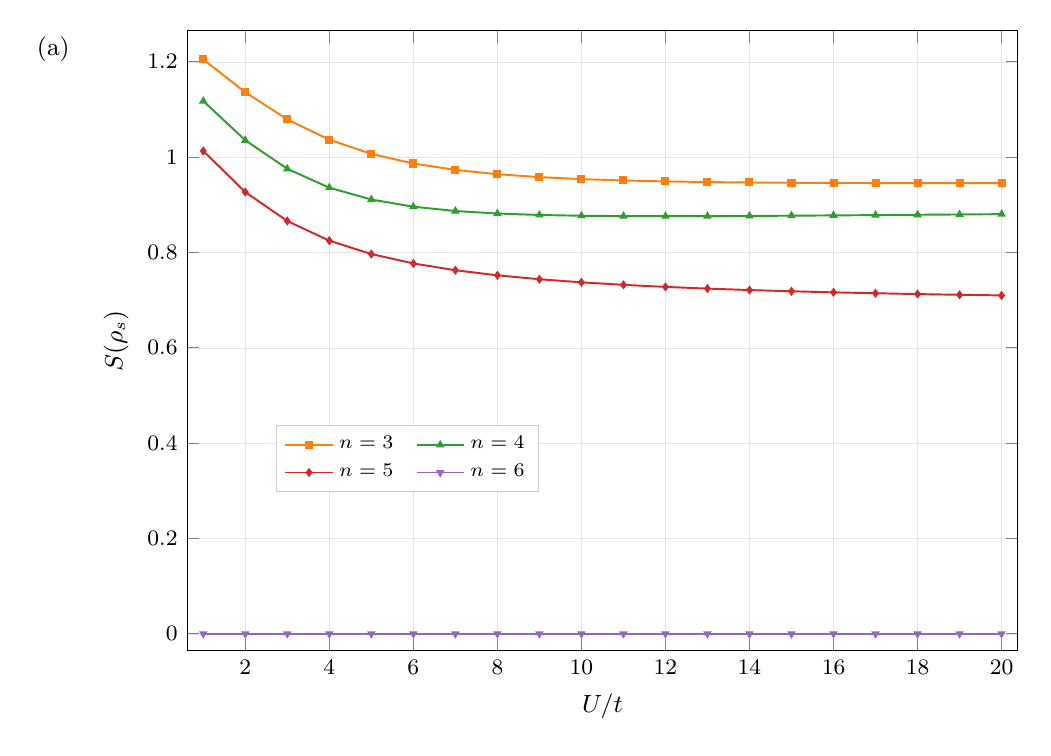
\begin{tikzpicture}
  \begin{axis}[
    width=\columnwidth,
    height=0.78\columnwidth,
    xlabel={$U/t$},
    ylabel={$S(\rho_s)$},
    grid=both,
    grid style={line width=.1pt, draw=gray!20},
    tick label style={font=\footnotesize\rmfamily, /pgf/number format/fixed},
    label style={font=\small\rmfamily},
    scaled ticks=false,
    legend style={font=\scriptsize\rmfamily, draw=gray!40, at={(0.5,1.03)}, anchor=south, /tikz/every even column/.append style={column sep=6pt}},
    legend cell align={left},
    legend columns=2,
    ymin=-0.036,
    ymax=1.265,
    xmin=0.62,
    xmax=20.38,
    legend style={at={(0.265,0.310)}, anchor=center, fill=white},
    after end axis/.append code={\node[anchor=east, font=\small\rmfamily] at (axis description cs:-0.13,0.970) {(a)};},
  ]
    \addplot[color=gmeC1, mark=square*, mark size=1.1pt, line width=0.7pt] coordinates {
        (1,1.204737) (2,1.135946) (3,1.078924) (4,1.03636)
        (5,1.006619) (6,0.986508) (7,0.973046) (8,0.964013)
        (9,0.957906) (10,0.953743) (11,0.950886) (12,0.948922)
        (13,0.947578) (14,0.946668) (15,0.946069) (16,0.945693)
        (17,0.945479) (18,0.945383) (19,0.945375) (20,0.94543)
    };
    \addlegendentry{$n=3$}
    \addplot[color=gmeC2, mark=triangle*, mark size=1.1pt, line width=0.7pt] coordinates {
        (1,1.117553) (2,1.035216) (3,0.975365) (4,0.935729)
        (5,0.91092) (6,0.895843) (7,0.886829) (8,0.881526)
        (9,0.878496) (10,0.876873) (11,0.876128) (12,0.875937)
        (13,0.876096) (14,0.876477) (15,0.876996) (16,0.877597)
        (17,0.878245) (18,0.878915) (19,0.879591) (20,0.880263)
    };
    \addlegendentry{$n=4$}
    \addplot[color=gmeC3, mark=diamond*, mark size=1.1pt, line width=0.7pt] coordinates {
        (1,1.012754) (2,0.926526) (3,0.865866) (4,0.824635)
        (5,0.79651) (6,0.776826) (7,0.762579) (8,0.751916)
        (9,0.743696) (10,0.737197) (11,0.731951) (12,0.727641)
        (13,0.724049) (14,0.721018) (15,0.718432) (16,0.716205)
        (17,0.714273) (18,0.712583) (19,0.711096) (20,0.709779)
    };
    \addlegendentry{$n=5$}
    \addplot[color=gmeC4, mark=triangle*, mark size=1.1pt, mark options={rotate=180}, line width=0.7pt] coordinates {
        (1,0) (2,0) (3,0) (4,0)
        (5,0) (6,0) (7,0) (8,0)
        (9,0) (10,0) (11,0) (12,0)
        (13,0) (14,0) (15,0) (16,0)
        (17,0) (18,0) (19,0) (20,0)
    };
    \addlegendentry{$n=6$}
  \end{axis}
\end{tikzpicture}
